\documentclass{article}

\usepackage{graphicx}
\usepackage{float}
\usepackage{caption}
\usepackage{subcaption}
\usepackage{multirow}
\usepackage{hyperref}
\hypersetup{
    colorlinks  = true,
    linkcolor   = blue,
    filecolor   = blue,      
    urlcolor    = blue,
}

\title{Student job report: Bootstrap high quantiles estimation.}
\author{Joris LIMONIER}
\date{February - May 2021}

\begin{document}
\maketitle

\newpage
\tableofcontents
\listoffigures
\newpage

\section{Introduction}
In this project we want to estimate the confidence we have when computing various quantiles. This task may be fairly straightforward when working with known distributions or arbitrary amounts of data but this seldom occurs in engineering or other real world applications. For this reason, here we try to accomplish that task on an unknown distribution and given limited amounts of data.

We define the n-th quantile as follows:
\begin{equation}
    q_n := 1 - 10^{-n}
\end{equation}
which gives $q_1 = 0.9$, $q_2 = 0.99$ ...etc. Where, simply speaking, $q_n$ represents ``0" followed by $n$ nines. For our applications, we are mostly interested in $q_3, q_4$ and $q_5$.

The data we work with is presented in figure \ref{fig: initial data} and plotted in the histogram in figure \ref{fig: visual representation of the initial data}.

\begin{figure}[H]
    \centering
    \begin{subfigure}{.25\textwidth}
        \centering
        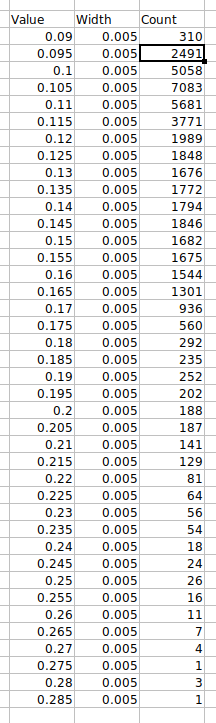
\includegraphics[width=\textwidth]{images/excel_data.png}
        \caption{Initial data}
        \label{fig: initial data}
    \end{subfigure}
    \hfill
    \begin{subfigure}{.74\textwidth}
        \centering
        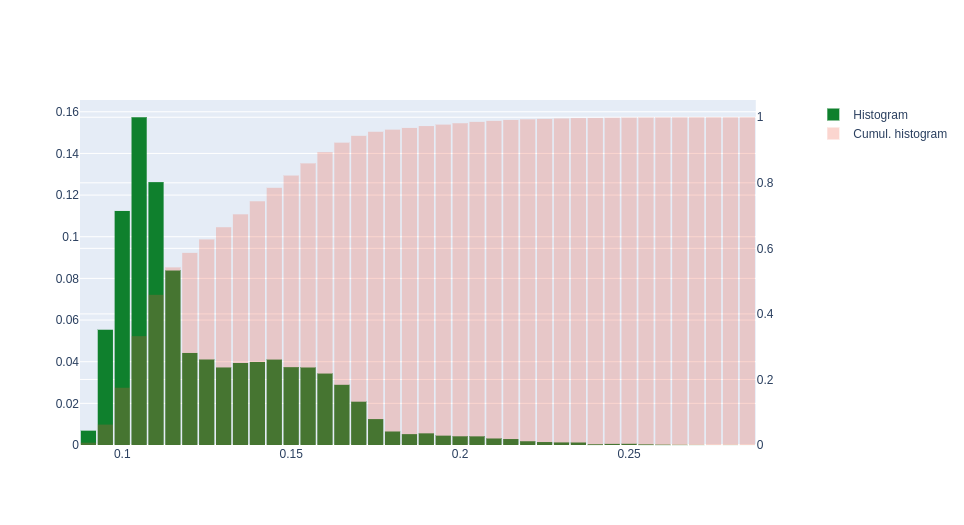
\includegraphics[width=\textwidth]{images/plot_excel_data.png}
        \caption{Visual representation of the initial data}
        \label{fig: visual representation of the initial data}
    \end{subfigure}
    \caption{A look at the initial data}
\end{figure}

\section{Bootstrap}
\label{section: bootstrap}
We use the bootstrap to estimate the confidence in the computed quantiles, even with small to moderate sample size.

Let \(n\) be the size of the data at our disposal and let \(q_k\) be the quantile we are interested in computer. Here is how we proceed:
\begin{enumerate}
    \item We draw a random sample of size \(n\) with replacement from our initial data.
    \item We compute \(q_k\) on the sample we just drew.
    \item We repeat the process over multiple runs.
    \item We compute the confidence intervals (details in section \ref{section: confidence intervals on the bootstrap})
\end{enumerate}

The plots in figure \ref{fig: estimation of quantiles} show the evolution of our estimate for the value of the quantiles as we go through runs of the bootstraps. The grey areas represent the $95\%$ confidence intervals during that evolution. We will see how to get the confidence intervals from our histogram in section \ref{section: confidence intervals on the bootstrap}.

\begin{figure}
    \centering
    \begin{subfigure}{.84\textwidth}
        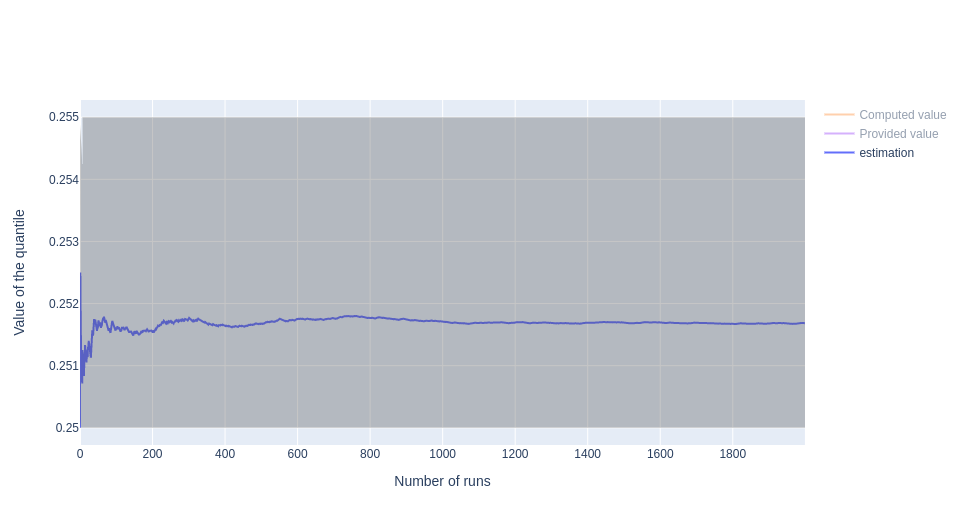
\includegraphics[width=\textwidth]{images/estimation_q3.png}
        \caption{Estimation of $q_3$}
    \end{subfigure}
    \hfill
    \begin{subfigure}{.84\textwidth}
        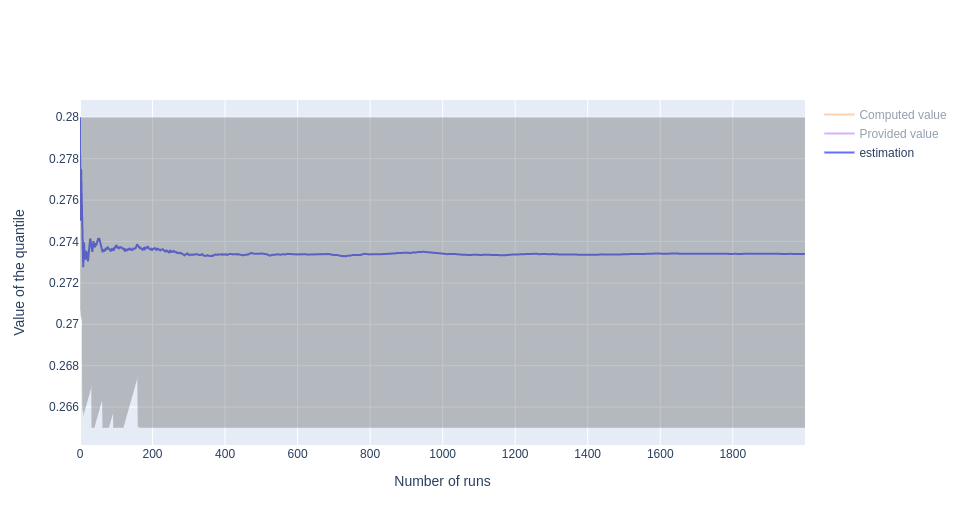
\includegraphics[width=\textwidth]{images/estimation_q4.png}
        \caption{Estimation of $q_4$}
    \end{subfigure}
    \hfill
    \begin{subfigure}{.84\textwidth}
        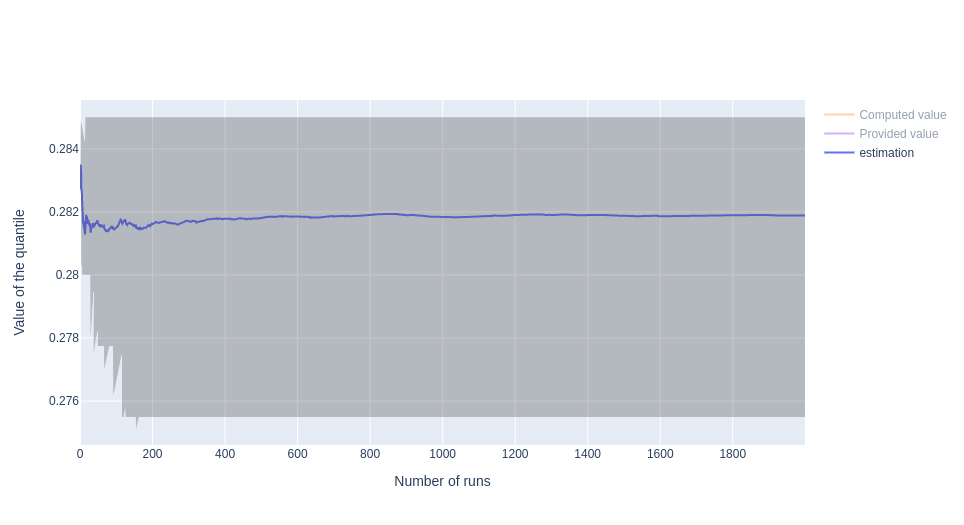
\includegraphics[width=\textwidth]{images/estimation_q5.png}
        \caption{Estimation of $q_5$}
    \end{subfigure}
    \caption{Estimation of the quantiles over bootstrap runs}
    \label{fig: estimation of quantiles}
\end{figure}

\section{Confidence intervals on the bootstrap}
\label{section: confidence intervals on the bootstrap}

Let us fix a quantile that we call $q$ that we want to estimate. The bootstrap consists of two parts:

\begin{enumerate}
    \item[Part 1] Take a random sample from our original data, and determine its value for $q$.
    \item[Part 2] Take all the $q$'s that have been computed for each individual sample and deduce $q$ and its confidence interval.
\end{enumerate}\

Part 1 is fairly straightforward so we will focus on the second part.

\paragraph{Estimating the quantile} Our estimation of the quantile $q$ for the underlying distribution is simply computed by taking the average of all the $q$'s of each individual sample.

\paragraph{Computing the confidence intervals} Let's say we want to compute the $95\%$ confidence interval. To do so, we take all the $q$'s that have been computed for each individual sample and sort them. Then we take the 0.025-th quantile as our lower bound for the confidence intervals and the 0.975-th quantile as our upper bound for the confidence intervals. \\
As one may expect, the values 0.025 and 0.975 are found as follows:
\[
    \frac{1 - 0.95}{2} = 0.025 \qquad \mbox{and} \qquad 1 - \frac{(1 - 0.95)}{2} = 0.975
\]
where the 0.95 comes from the $95\%$ confidence interval. \\
More generally, for a confidence level of $\gamma$ (instead of $95\%$), one has that the lower and upper bounds of the confidence interval are respectively
\[
    \gamma_{lo} := \frac{1 - \gamma}{2} \qquad \mbox{and} \qquad \gamma_{up} := 1 - \frac{(1 - \gamma)}{2}
\]

\section{Fine tuning}
Let us assume that we are working with a given data set and we have no way of getting new or more reliable data. We are trying to get the quantiles as precisely as possible and with confidence intervals as small as possible.

There are two parameters of the bootstrap that we can adjust to meet our goals
\begin{enumerate}
    \item The size of the resamples.
    \item The number of resamples.
\end{enumerate}\

We touched on the number of resamples already in section \ref{section: bootstrap}, however we haven't dicussed the size of the resamples.

What impact would increasing the size of the resamples have ? The only time it comes into play is when we take the quantiles of the resamples. Then, what would happen if we took the quantiles of a resample of different size ? Taking the quantile of a smaller resample likely means that we will have less \textit{refinement}. That is, our quantiles at each resample would likely take a smaller set of values. This is further explained by the way we proceed if we have sparse values, which is our case since we work with ``high" quantiles (where we have few values available).

\textbf{According to our data}, it seems that there is close to no change in the estimation of the quantiles after $1000$ repetitions of the bootstrap. The variations are small after 500 runs already but for safety purposes we consider that we have our final guess after 1000 runs. As for the confidence intervals, only in some edge cases do we have changes past the 1000 mark. \\
\textit{NB: Our estimate of 1000 runs is based on empirical evidence. It is not a theoretical result, however, we believe that it is suitable for engineering purposes.}

% \begin{center}
%     \begin{tabular}{|c|c|c|c|}
%         \hline
%                 & \multicolumn{3}{c|}{Quantile}                        \\
%         \hline
%                 & q3                           & q4       & q5        \\
%         \hline
%         100     & 0.076622                     & 0.079702 & 0.0799506 \\
%         1000    & 0.040009                     & 0.051016 & 0.0546004 \\
%         10000   & 0.015000                     & 0.020000 & 0.0249999 \\
%         100 000 & 0.005000                     & 0.010000 & 0.0049999 \\
%         \hline
%     \end{tabular}
% \end{center}









\end{document}